\chapter{Navigation Client}
Der \texttt{Studmap.Navigator} ist eine Android App, welche den Navigationsservice auf Smartphones und Tablets bereitstellen soll. Dem Anwender sollen folgende Funktionen zu Verf�gung gestellet werden:
\begin{itemize}
\item Anzeige der Karte einzelner Stockwerken
\item Eingabe von Start- und/oder Zielpunkt
\item Ermittlung der aktuellen Position
\item Navigation zum Zielpunkt
\item Suchen und Anzeigen von POI's
\item Anmeldung am Server
\end{itemize}

\section{Struktur}
Bei der App handelt es sich um eine Mischung aus nativer und Container-App.
Eine Container-App stellt dabei innerhalb eines nativen Android Rahmens Webseiten und Services zur Verf�gung. In diesem Projekt handelt es sich dabei vor allem um die Karten und die Navigation. Diese werden mit Hilfe der JavaScript-Bibliothek D3 dargestellt und bedient.
Alle weiteren Funktionen des Clients werden nativ erstellt. Hierbei sei vor allem die Benutzeranmeldung, sowie die Suche nach POI's oder Zielpunkten genannt.

\section{Design}
Das Design einer App sollte m�glichst einfach, funktional und �bersichtlich sein. Diese Ziele wurden auch hier verfolgt. Als Vorbild f�r das Design diente Maps von Google, woraus viele Ideen eingeflossen sind. Um die Designideen darzustellen wurden die im folgenden Bild dargestellten MockUps erstellt.
\begin{figure}
\centering
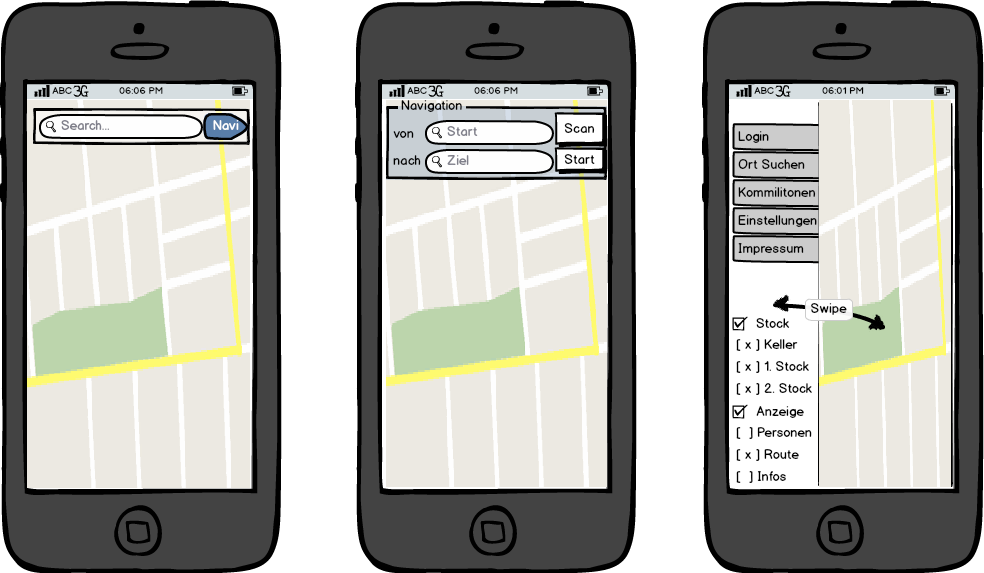
\includegraphics[width=0.7\linewidth]{C:/Users/Marcus/Documents/Visual Studio 2012/Projects/StudMap/doku/Bilder/Mockups}
\caption{}
\label{fig:Mockups}
\end{figure}

